\documentclass{beamer}
\usetheme{Hannover}
\usepackage[utf8x]{inputenc}
\usepackage[T1]{fontenc}
\usepackage{default}
\hypersetup{pdftitle=RicochetRobots}
\hypersetup{pdfpagemode=FullScreen}
\usepackage{color}
\definecolor{light-gray}{gray}{0.55}
\definecolor{blue-gray}{RGB}{214, 214, 240}
\usepackage[footheight=1em]{beamerthemeboxes}
\addfootboxtemplate{\color{blue-gray}}{\color{white}
     \hfill\insertframenumber/\inserttotalframenumber\hspace{2em}\null}



\title{
\centering{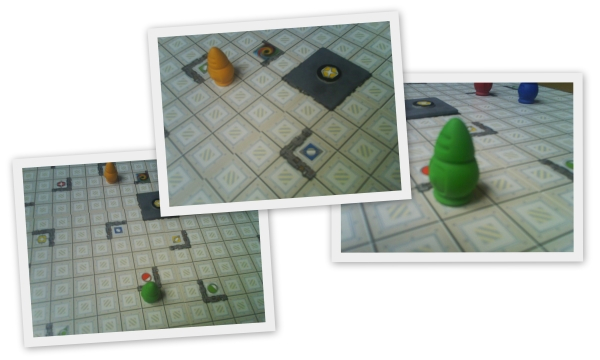
\includegraphics[width=\linewidth]{img/Ricochet_Robots.png}}
\raggedleft{Ricochet Robots}
}


\begin{document}

\begin{frame}[plain]
\vspace{3em}
\titlepage
\end{frame}

\begin{frame}[plain]
\frametitle{Plan}
\tableofcontents
\end{frame}


\section{Pr\'esentation}

\begin{frame}
\setcounter{framenumber}{1}
  \vfill
  \begin{center}
    \Large{Construction des chemins possibles pour \'evaluer l'atteignabilit\'e de la cible.}\vfill
\pause 
\normalsize{\textit{id\'ee :} en construisant la carte des d\'eplacements possibles de chacun des robots, est-il possible d'\'evaluer le plus court chemin vers la cible ?}
  \end{center}
  \vfill
\end{frame}

\section{Construction de la carte routi\`ere}

\subsection{Initialisation}

\begin{frame}
  \begin{tabular}{l}
  \hspace{-.1cm}g\'en\'eration $\leftarrow 0$\\
  \\
  \hspace{-.1cm}Pour i de 1 \`a (nombre de robots) faire\\
    \begin{tabular*}{\textwidth}{|p{.5\textwidth}}
    \hspace{-.1cm}Pour chaque direction autoris\'ee pour le robot faire\\
      \begin{tabular}{|l}
      Cr\'eer un clone\\
      Propager(clone, g\'en\'eration)\\
      \end{tabular}
      \\Masquer robot \color{light-gray}{\textit{// Pour que le robot r\'eel ne soit pas consid\'er\'e comme un obstacle pendant l'exploration}}
    \end{tabular*}
  \end{tabular}
\end{frame}


\subsection{Propagation}

\begin{frame}
  \textbf{Propager(clone, g\'en\'eration)}\\
  \begin{tabular}{l}
    \hspace{-.1cm}Tant que le clone n'est pas bloqu\'e faire\\
    \begin{tabular}{|l}
      $case_{i,j} \leftarrow min(generation,case_{i,j})$
    \end{tabular}
    \\ \hspace{-.1cm}FinTq \color{light-gray}{\textit{// le robot est arr\^et\'e}}\\
    \color{black}\\
    \hspace{-.1cm}Si $case_{i,j} >$ g\'en\'eration\\
    \hspace{-.1cm}Alors\\
      \begin{tabular}{|l}
        $case_{i,j} \leftarrow$ g\'en\'eration\\
        D\'etruire le clone\\
        g\'en\'eration $\leftarrow$ g\'en\'eration + 1\\
        \\
        \hspace{-.1cm}Pour chaque direction autoris\'ee pour le clone faire\\
        \begin{tabular}{|l}
          Cr\'eer clone\\
          Propager(clone, g\'en\'eration)\\
        \end{tabular}
      \end{tabular}
    \\ \hspace{-.1cm}\color{light-gray}{\textit{// Sinon ne rien faire}}\\\color{black}
  \end{tabular}
\end{frame}

\subsection{Co\^ut}

\begin{frame}
  \vfill
  \begin{center}
    temps : $O(3^n)$\\
    n : nombre total de g\'en\'erations produites
    \vfill
    m\'emoire : $O(l^2)$\\
    l : taille d'un c\^ot\'e de la matrice
  \end{center}
  \vfill
\end{frame}

\subsection{Alternative}

\begin{frame}
  \vfill
  \centering{Faut-il considérer tous les chemins, ou bien se limiter à ceux qui n'ont pas été parcourus ?}
  \vfill
\end{frame}

\begin{frame}
 \begin{description}
  \item[Lemme : ] lorsqu'un robot s'arrête sur une case atteignable \footnote{case où un robot peut s'arrêter} par un autre robot, il peut parcourir toute la carte de l'autre robot.
 \end{description}
\end{frame}

\begin{frame}
  \begin{figure}[htbp]
    \centering
    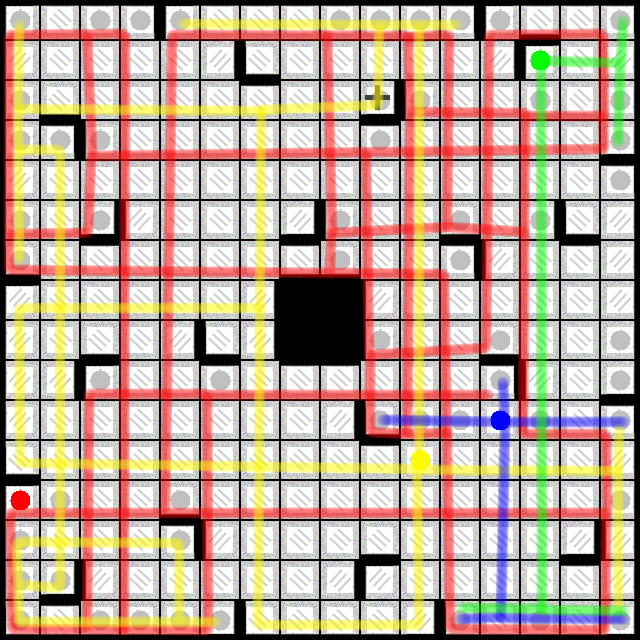
\includegraphics[width=.7\linewidth]{img/chemins_initiaux.png}
    \caption{Cartographie simplifi\'ee}
  \end{figure}
\end{frame}

\section{Recherche de solution}
\begin{frame}
  \vfill
  \centering Recherche de solution
  \vfill
\end{frame}

\subsection{Recherche \`a partir de la cible}
\begin{frame}
\begin{tabular}{l}
\hspace{-.1cm}g\'en\'eration $\leftarrow 0$\\
\\
\hspace{-.1cm}Pour chaque direction disponible faire\\
  \begin{tabular}{|l}
  Cr\'eer un clone\\
  Explore(clone, g\'en\'eration)\\
  \end{tabular}
  \\Masquer robot
\end{tabular} 
\end{frame}

\subsection{Exploration}
\begin{frame}
 \begin{tabular*}{\textwidth}{p{.7\textwidth}}
\hspace{-.1cm}$mem$ : tableau d'entiers\\
\hspace{-.1cm}$choix \in M_{i,j} \times \mathbb{N}$\\
\hspace{-.1cm}$i = 0$\\
\\
\hspace{-.1cm}Tant que le clone n'est pas bloqu\'e faire\\
  \begin{tabular}{|l}
    Si $(M_{i,j}$ atteignable par $R_{cible})$ et $(\exists R_c | M_{i,j}$ atteignable par $R_c)$\\
    Alors $mem[i] \leftarrow (M_{i,j},d(M_{i,j},R_c))$\\
    Avancer\\
  \end{tabular}
%\\$choix \leftarrow min(mem)[0]$ \comment{r\'ecup\'eration de la case o\`u se trouve la distance minimale}
\end{tabular*}
%\comment{Ici, choix correspond \`a la case o\`u $\left(R_{c_{i,j}} | c \neq couleur(R_c)\right)$ pourra venir bloquer $R_{cible}$}
\begin{tabular*}{\textwidth}{p{.7\textwidth}}
  \\
  \hspace{-.1cm}Trier $mem$ par $d(M_{i,j},R_c)$ croissant.\\
  \hspace{-.1cm}$tmp \leftarrow M_{i,j} + max \left( d(M_{i,j},R_c) \right)$\\
  \\
  \hspace{-.1cm}Pour i de 1 \`a $|mem|$ faire\\
  \begin{tabular*}{\textwidth}{|p{.7\textwidth}}
    Si $(M_{i,j} + d(M_{i,j},R_c)) < tmp$\\
    Alors\\
    \begin{tabular*}{\textwidth}{|p{.7\textwidth}}
      $tmp \leftarrow min(tmp,M_{i,j} + d(M_{i,j},R_c)  + d(M_{i,j},C_{i,j}))$\\
    \end{tabular*}
  \end{tabular*}
\end{tabular*}
\end{frame}



\end{document}
